\documentclass[aspectratio=169,11pt]{beamer}

\usetheme{Madrid}
\usecolortheme{default}
\setbeamertemplate{navigation symbols}{}
\setbeamertemplate{footline}[frame number]

\usepackage{amsmath,amssymb}
\usepackage{graphicx}
\usepackage{tikz}
\usetikzlibrary{positioning,calc}
\usetikzlibrary{arrows.meta,decorations.pathmorphing}

\definecolor{RamRed}{RGB}{190,40,45}
\definecolor{RamBlue}{RGB}{30,90,180}
\definecolor{SoftGray}{RGB}{245,245,245}
\definecolor{DarkGray}{RGB}{70,70,70}
\definecolor{MapGreen}{RGB}{48,150,95}
\definecolor{MapGold}{RGB}{235,180,45}

\setbeamercolor{title}{fg=DarkGray}
\setbeamercolor{frametitle}{fg=white,bg=RamBlue}
\setbeamercolor{structure}{fg=RamBlue}

\tikzset{
  v/.style={circle,draw=black,fill=white,inner sep=1.8pt},
  edge/.style={draw=RamBlue,line width=1.25pt},
  topic/.style={draw=black!30,fill=SoftGray,rounded corners=5pt,inner sep=7pt,
    text width=5.8cm,minimum height=1.65cm,align=left},
}


\usepackage{booktabs}
\tikzset{dot/.style={circle,fill=black,inner sep=2pt}, lab/.style={circle,draw=black,fill=white,inner sep=2pt,minimum size=6mm,font=\small},selected/.style={draw=RamRed,line width=2pt}}

\newcommand{\Def}[2]{\begin{block}{#1}#2\end{block}}
\newcommand{\Thm}[2]{\begin{block}{#1}#2\end{block}}
\renewcommand{\Proof}[1]{\begin{block}{Proof}\normalsize #1\end{block}}
\newcommand{\Question}[1]{\begin{block}{Question}#1\end{block}}
\renewcommand{\Example}[1]{\begin{block}{Example}#1\end{block}}
\newcommand{\fall}[2]{#1^{\underline{#2}}}
\newcommand{\rise}[2]{#1^{\overline{#2}}}
\newcommand{\stir}[2]{\left\{\begin{matrix}#1\\#2\end{matrix}\right\}}
\newcommand{\cyc}[2]{\left[\begin{matrix}#1\\#2\end{matrix}\right]}
\newcommand{\eul}[2]{\left\langle\begin{matrix}#1\\#2\end{matrix}\right\rangle}
\newcommand{\coef}[2]{[#1^{#2}]}
\newcommand{\gap}{\par\medskip}

\title{Planarity}
\author{Jeremy Quastel}\date{}\begin{document}
\begin{frame}[plain]\begin{center}{\Huge\bfseries Planarity}\par\vspace{.25cm}{\Large Section 1.5}\par\vspace{.15cm}{\large Harris--Hirst--Mossinghoff, \emph{Combinatorics and Graph Theory}}\par\vspace{.1cm}\resizebox{!}{2.7cm}{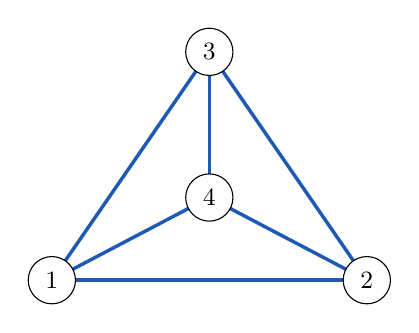
\begin{tikzpicture}[scale=1]
\coordinate (v1) at (-2.000,-1.300);
\coordinate (v2) at (2.000,-1.300);
\coordinate (v3) at (0.000,1.600);
\coordinate (v4) at (0.000,-0.250);
\draw[edge] (v1)--(v2);
\draw[edge] (v1)--(v3);
\draw[edge] (v1)--(v4);
\draw[edge] (v2)--(v3);
\draw[edge] (v2)--(v4);
\draw[edge] (v3)--(v4);
\node[lab] at (v1) {1};
\node[lab] at (v2) {2};
\node[lab] at (v3) {3};
\node[lab] at (v4) {4};
\end{tikzpicture}}\par\vspace{.25cm}Jeremy Quastel\end{center}\end{frame}
\begin{frame}[plain]\large \begin{center}{\Huge\bfseries Today\textquotesingle s lecture}\par\vspace{.5cm}\end{center}\begin{columns}[c,onlytextwidth]\begin{column}{.48\textwidth}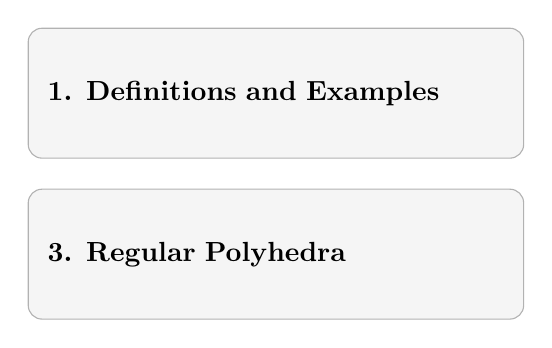
\begin{tikzpicture}\node[topic](a){\textbf{1. Definitions and Examples}};\node[topic,below=.38cm of a]{\textbf{3. Regular Polyhedra}};\end{tikzpicture}\end{column}\begin{column}{.48\textwidth}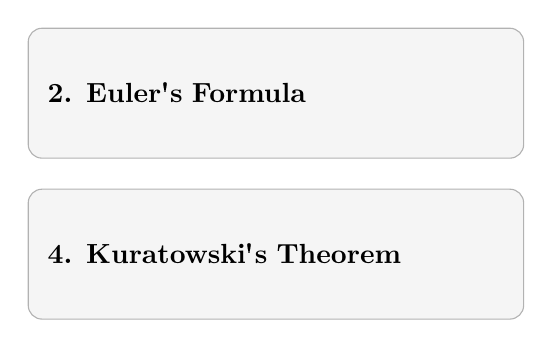
\begin{tikzpicture}\node[topic](a){\textbf{2. Euler\textquotesingle s Formula}};\node[topic,below=.38cm of a]{\textbf{4. Kuratowski\textquotesingle s Theorem}};\end{tikzpicture}\end{column}\end{columns}\end{frame}
\begin{frame}{Can We Draw This Graph Without Crossings?}
\large
\Question{The drawing below has crossing edges. Does the graph have to be drawn this way?}
\begin{center}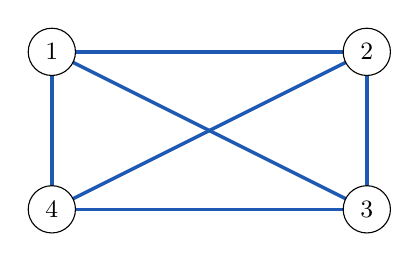
\begin{tikzpicture}[scale=1]
\coordinate (v1) at (-2.000,1.000);
\coordinate (v2) at (2.000,1.000);
\coordinate (v3) at (2.000,-1.000);
\coordinate (v4) at (-2.000,-1.000);
\draw[edge] (v1)--(v2);
\draw[edge] (v1)--(v3);
\draw[edge] (v1)--(v4);
\draw[edge] (v2)--(v3);
\draw[edge] (v2)--(v4);
\draw[edge] (v3)--(v4);
\node[lab] at (v1) {1};
\node[lab] at (v2) {2};
\node[lab] at (v3) {3};
\node[lab] at (v4) {4};
\end{tikzpicture}\end{center}
\end{frame}
\begin{frame}{The Same Graph, Drawn Differently}
\large
\begin{center}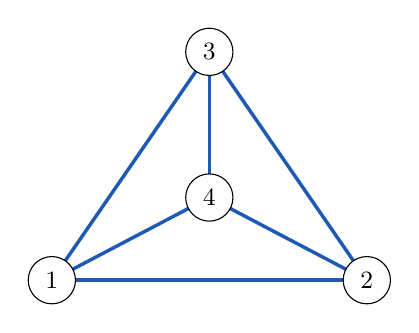
\begin{tikzpicture}[scale=1]
\coordinate (v1) at (-2.000,-1.300);
\coordinate (v2) at (2.000,-1.300);
\coordinate (v3) at (0.000,1.600);
\coordinate (v4) at (0.000,-0.250);
\draw[edge] (v1)--(v2);
\draw[edge] (v1)--(v3);
\draw[edge] (v1)--(v4);
\draw[edge] (v2)--(v3);
\draw[edge] (v2)--(v4);
\draw[edge] (v3)--(v4);
\node[lab] at (v1) {1};
\node[lab] at (v2) {2};
\node[lab] at (v3) {3};
\node[lab] at (v4) {4};
\end{tikzpicture}\end{center}
The graph is still $K_4$: every pair of vertices is adjacent.
\gap We have changed the drawing, not the graph.
\end{frame}
\begin{frame}{Definition: Planar Graph and Plane Graph}
\large
\Def{Planar graph}{A graph is \textbf{planar} if it has a drawing in the plane in which edges meet only at common endpoints.}
\Def{Plane graph}{A particular crossing-free drawing is a \textbf{plane embedding} of the graph.}
\gap A crossing in one drawing does not establish nonplanarity.
\end{frame}
\begin{frame}{Example: A Plane Drawing of the Cube}
\large
\begin{center}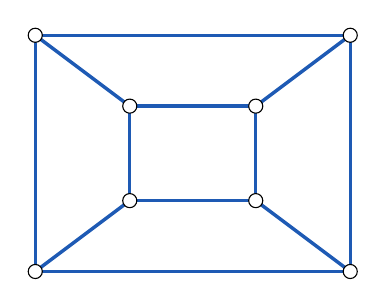
\begin{tikzpicture}[scale=1]
\coordinate (v1) at (-2.000,-1.500);
\coordinate (v2) at (2.000,-1.500);
\coordinate (v3) at (2.000,1.500);
\coordinate (v4) at (-2.000,1.500);
\coordinate (v5) at (-0.800,-0.600);
\coordinate (v6) at (0.800,-0.600);
\coordinate (v7) at (0.800,0.600);
\coordinate (v8) at (-0.800,0.600);
\draw[edge] (v1)--(v2);
\draw[edge] (v2)--(v3);
\draw[edge] (v3)--(v4);
\draw[edge] (v4)--(v1);
\draw[edge] (v5)--(v6);
\draw[edge] (v6)--(v7);
\draw[edge] (v7)--(v8);
\draw[edge] (v8)--(v5);
\draw[edge] (v1)--(v5);
\draw[edge] (v2)--(v6);
\draw[edge] (v3)--(v7);
\draw[edge] (v4)--(v8);
\node[v] at (v1) {};
\node[v] at (v2) {};
\node[v] at (v3) {};
\node[v] at (v4) {};
\node[v] at (v5) {};
\node[v] at (v6) {};
\node[v] at (v7) {};
\node[v] at (v8) {};
\end{tikzpicture}\end{center}
\Question{Count its vertices and edges. How many regions does the drawing divide the plane into?}
\end{frame}
\begin{frame}{Definition: Regions and Boundaries}
\large
\Def{Region (face)}{A connected component of the plane left after removing the embedded graph. The unbounded component is also a region.}
\Def{Boundary length}{The number of edge occurrences in a walk around the boundary, counted with multiplicity.}
\gap A bridge can occur twice on the boundary of one region.
\end{frame}
\begin{frame}{Counting the Regions of the Cube}
\large
\begin{center}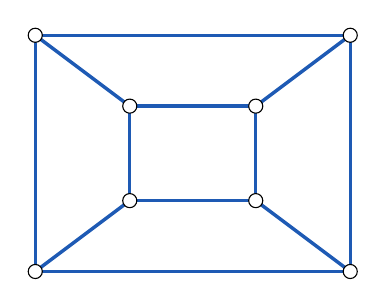
\begin{tikzpicture}[scale=1]
\coordinate (v1) at (-2.000,-1.500);
\coordinate (v2) at (2.000,-1.500);
\coordinate (v3) at (2.000,1.500);
\coordinate (v4) at (-2.000,1.500);
\coordinate (v5) at (-0.800,-0.600);
\coordinate (v6) at (0.800,-0.600);
\coordinate (v7) at (0.800,0.600);
\coordinate (v8) at (-0.800,0.600);
\draw[edge] (v1)--(v2);
\draw[edge] (v2)--(v3);
\draw[edge] (v3)--(v4);
\draw[edge] (v4)--(v1);
\draw[edge] (v5)--(v6);
\draw[edge] (v6)--(v7);
\draw[edge] (v7)--(v8);
\draw[edge] (v8)--(v5);
\draw[edge] (v1)--(v5);
\draw[edge] (v2)--(v6);
\draw[edge] (v3)--(v7);
\draw[edge] (v4)--(v8);
\node[v] at (v1) {};
\node[v] at (v2) {};
\node[v] at (v3) {};
\node[v] at (v4) {};
\node[v] at (v5) {};
\node[v] at (v6) {};
\node[v] at (v7) {};
\node[v] at (v8) {};
\end{tikzpicture}\end{center}
There are $8$ vertices, $12$ edges, and $6$ regions, including the outside.
\[8-12+6=2.\]
\end{frame}
\begin{frame}{Why Boundary Edges Must Be Counted with Multiplicity}
\large
\Example{A tree with $m$ edges has just one region. Each edge has both sides on that region, so its boundary length is $2m$.}
\gap Each edge has two sides. They may belong to two different regions or to the same region.
\[\sum_{R} b(R)=2m.\]
\end{frame}
\begin{frame}{Theorem: Euler's Formula}
\large
\Thm{Euler's Formula}{For a connected plane graph with $n$ vertices, $m$ edges, and $f$ regions,\[n-m+f=2.\]}
\gap The number of regions is therefore determined by the abstract graph once a plane embedding exists.
\end{frame}
\begin{frame}{Proof of Euler's Formula: The Tree Case}
\large
\Thm{Recall}{A tree with $n$ vertices has $n-1$ edges.}
\Proof{A plane tree has no cycle enclosing a region, so it has only the unbounded region. Thus $f=1$, and\[n-m+f=n-(n-1)+1=2.\]This includes the single-vertex tree.}
\end{frame}
\begin{frame}{Proof Continued: Removing a Cycle Edge}
\large
\Proof{If the connected plane graph is not a tree, choose an edge $e$ on a cycle. It is not a bridge, so deleting it preserves connectedness.\gap Its two sides border distinct regions. Deleting $e$ merges those regions: $m$ and $f$ both decrease by one, while $n$ is unchanged.\gap Hence $n-m+f$ is unchanged. Repeat until a tree remains; its value is $2$.\hfill$\square$}
\end{frame}
\begin{frame}{Euler's Formula: A Worked Example}
\large
\Question{A connected plane graph has $12$ vertices and $18$ edges. How many regions does it have?}
\[f=2-n+m=2-12+18=8.\]
\gap If another crossing-free drawing of the same graph looks very different, it still has eight regions.
\end{frame}
\begin{frame}{Disconnected Plane Graphs}
\large
\Thm{Extension}{If a plane graph has $c$ connected components, then\[n-m+f=1+c.\]}
\Proof{Join the components by $c-1$ new edges without crossings. Each new edge is a bridge and creates no new region. Apply Euler's formula to the resulting connected graph:\[n-(m+c-1)+f=2.\]Rearrange.\hfill$\square$}
\end{frame}
\begin{frame}{Counting Edge Sides}
\large
\Thm{Boundary identity}{For every plane graph,\[\sum_R b(R)=2m.\]}
\gap In a connected simple plane graph with $n\ge3$, every region has boundary length at least $3$.
\[3f\le 2m.\]
\gap This combines a local observation about faces with Euler's global formula.
\end{frame}
\begin{frame}{Theorem: An Edge Bound for Planar Graphs}
\large
\Thm{Planar edge bound}{A simple planar graph with $n\ge3$ vertices has at most $3n-6$ edges.}
\Proof{First assume connectedness and choose a plane embedding. Euler gives $f=2-n+m$, while $3f\le2m$. Thus\[3(2-n+m)\le2m,\qquad m\le3n-6.\]If the graph is disconnected, add crossing-free edges to connect it and apply the connected case.\hfill$\square$}
\end{frame}
\begin{frame}{The Complete Graph on Five Vertices}
\large
\begin{center}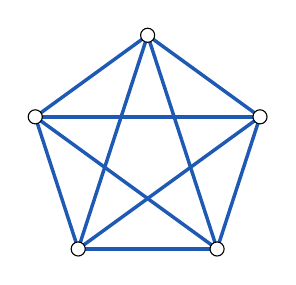
\begin{tikzpicture}[scale=1]
\coordinate (v1) at (0.000,1.500);
\coordinate (v2) at (-1.427,0.464);
\coordinate (v3) at (-0.882,-1.214);
\coordinate (v4) at (0.882,-1.214);
\coordinate (v5) at (1.427,0.464);
\draw[edge] (v1)--(v2);
\draw[edge] (v1)--(v3);
\draw[edge] (v1)--(v4);
\draw[edge] (v1)--(v5);
\draw[edge] (v2)--(v3);
\draw[edge] (v2)--(v4);
\draw[edge] (v2)--(v5);
\draw[edge] (v3)--(v4);
\draw[edge] (v3)--(v5);
\draw[edge] (v4)--(v5);
\node[v] at (v1) {};
\node[v] at (v2) {};
\node[v] at (v3) {};
\node[v] at (v4) {};
\node[v] at (v5) {};
\end{tikzpicture}\end{center}
\Question{Could a different drawing remove all crossings?}
$K_5$ has $n=5$ and $m=10$, whereas $3n-6=9$.
\gap Therefore $K_5$ is not planar.
\end{frame}
\begin{frame}{A Stronger Bound Without Triangles}
\large
\Thm{Triangle-free planar edge bound}{If $G$ is simple, planar, triangle-free, and $n\ge3$, then\[m\le2n-4.\]}
\Proof{In a connected plane embedding, every facial boundary has length at least four. Thus $4f\le2m$. Substitute $f=2-n+m$ and rearrange. Disconnected graphs can be joined by bridges without creating triangles.\hfill$\square$}
\end{frame}
\begin{frame}{The Three Utilities Problem}
\large
\begin{center}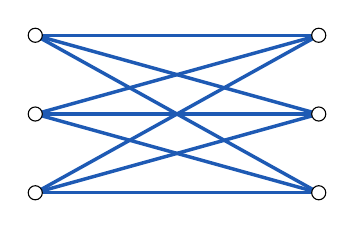
\begin{tikzpicture}[scale=1]
\coordinate (vx1) at (-1.800,1.000);
\coordinate (vx2) at (-1.800,0.000);
\coordinate (vx3) at (-1.800,-1.000);
\coordinate (vy1) at (1.800,1.000);
\coordinate (vy2) at (1.800,0.000);
\coordinate (vy3) at (1.800,-1.000);
\draw[edge] (vx1)--(vy1);
\draw[edge] (vx1)--(vy2);
\draw[edge] (vx1)--(vy3);
\draw[edge] (vx2)--(vy1);
\draw[edge] (vx2)--(vy2);
\draw[edge] (vx2)--(vy3);
\draw[edge] (vx3)--(vy1);
\draw[edge] (vx3)--(vy2);
\draw[edge] (vx3)--(vy3);
\node[v] at (vx1) {};
\node[v] at (vx2) {};
\node[v] at (vx3) {};
\node[v] at (vy1) {};
\node[v] at (vy2) {};
\node[v] at (vy3) {};
\end{tikzpicture}\end{center}
\Question{Can each of three houses be connected to each of three utilities without any crossings?}
The required graph is $K_{3,3}$.
\end{frame}
\begin{frame}{Why the Three Utilities Cannot Be Connected}
\large
\Proof{$K_{3,3}$ is bipartite, so it has no triangle. It has $n=6$ vertices and $m=9$ edges. If it were planar, the triangle-free bound would give\[9\le2(6)-4=8,\]a contradiction.\hfill$\square$}
\gap The obstruction is independent of how the houses and utilities are placed.
\end{frame}
\begin{frame}{The Edge Bound Is Necessary, Not Sufficient}
\large
\Question{Does $m\le3n-6$ imply that a graph is planar?}
No. $K_{3,3}$ satisfies $9\le12$, but is not planar.
\gap We need structural obstructions as well as numerical bounds.
\end{frame}
\begin{frame}{Theorem: A Vertex of Small Degree}
\large
\Thm{Degree bound}{Every nonempty simple planar graph has a vertex of degree at most $5$.}
\Proof{The cases $n\le2$ are immediate. For $n\ge3$,\[\frac1n\sum_{v}\deg(v)=\frac{2m}{n}\le6-\frac{12}{n}<6.\]If every degree were at least six, the average would be at least six.\hfill$\square$}
\end{frame}
\begin{frame}{What Happens When Equality Holds?}
\large
\Thm{Triangulations}{For a connected simple plane graph with $n\ge3$, equality $m=3n-6$ holds exactly when every facial boundary has length three.}
\Proof{The only inequality in the edge-bound proof was $3f\le2m$. Equality means every term in $\sum_R b(R)$ is exactly $3$.\hfill$\square$}
\end{frame}
\begin{frame}{A Bound Using the Girth}
\large
\Def{Girth}{The length of a shortest cycle.}
\Thm{Girth bound}{For a connected simple plane graph containing a cycle and having girth $g$,\[m\le\frac{g}{g-2}(n-2).\]}
\Proof{Every facial boundary has length at least $g$, so $gf\le2m$. Combine this with $f=2-n+m$ and solve for $m$.\hfill$\square$}
\end{frame}
\begin{frame}{Graphs on Polyhedra}
\large
A convex polyhedron determines a plane graph: choose a face as the outside and project its edges onto the plane.
\begin{center}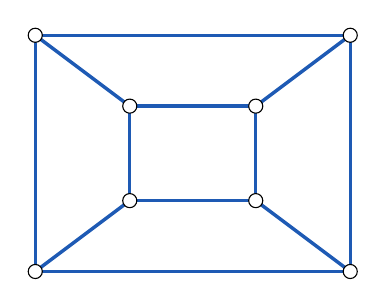
\begin{tikzpicture}[scale=1]
\coordinate (v1) at (-2.000,-1.500);
\coordinate (v2) at (2.000,-1.500);
\coordinate (v3) at (2.000,1.500);
\coordinate (v4) at (-2.000,1.500);
\coordinate (v5) at (-0.800,-0.600);
\coordinate (v6) at (0.800,-0.600);
\coordinate (v7) at (0.800,0.600);
\coordinate (v8) at (-0.800,0.600);
\draw[edge] (v1)--(v2);
\draw[edge] (v2)--(v3);
\draw[edge] (v3)--(v4);
\draw[edge] (v4)--(v1);
\draw[edge] (v5)--(v6);
\draw[edge] (v6)--(v7);
\draw[edge] (v7)--(v8);
\draw[edge] (v8)--(v5);
\draw[edge] (v1)--(v5);
\draw[edge] (v2)--(v6);
\draw[edge] (v3)--(v7);
\draw[edge] (v4)--(v8);
\node[v] at (v1) {};
\node[v] at (v2) {};
\node[v] at (v3) {};
\node[v] at (v4) {};
\node[v] at (v5) {};
\node[v] at (v6) {};
\node[v] at (v7) {};
\node[v] at (v8) {};
\end{tikzpicture}\end{center}
\gap Vertices, edges, and faces correspond to those of the polyhedron.
\end{frame}
\begin{frame}{Euler's Formula for Polyhedra}
\large
\Thm{Polyhedral Euler formula}{A convex polyhedron with $V$ vertices, $E$ edges, and $F$ faces satisfies\[V-E+F=2.\]}
\Example{For a cube: $V=8$, $E=12$, $F=6$. For a tetrahedron: $V=4$, $E=6$, $F=4$.}
\end{frame}
\begin{frame}{Definition: Regular Polyhedron}
\large
\Def{Regular polyhedron}{A convex polyhedron whose faces are congruent regular polygons, with the same number of faces meeting at every vertex.}
Suppose each face has $p$ edges and each vertex has degree $q$.
\[pF=2E,\qquad qV=2E.\]
Both $p$ and $q$ are at least $3$.
\end{frame}
\begin{frame}{Classifying the Possible Regular Polyhedra}
\large
Substitute $V=2E/q$ and $F=2E/p$ into Euler's formula:
\[\frac{2E}{q}-E+\frac{2E}{p}=2.\]
Consequently,
\[\frac1p+\frac1q>\frac12.\]
\Question{Which integer pairs $p,q\ge3$ satisfy this inequality?}
\end{frame}
\begin{frame}{Only Five Pairs Are Possible}
\large
If $p,q\ge4$, then $1/p+1/q\le1/2$. Thus one equals $3$.
\gap If $p=3$, the inequality gives $q<6$, so $q=3,4,5$.
\gap Interchanging $p$ and $q$ gives the remaining possibilities:
\[(3,3),(3,4),(4,3),(3,5),(5,3).\]
\end{frame}
\begin{frame}{The Five Platonic Solids}
\large
\renewcommand{\arraystretch}{1.35}
\begin{center}\begin{tabular}{lccrrr}\toprule Solid & $p$ & $q$ & $V$ & $E$ & $F$\\\midrule Tetrahedron&3&3&4&6&4\\Cube&4&3&8&12&6\\Octahedron&3&4&6&12&8\\Dodecahedron&5&3&20&30&12\\Icosahedron&3&5&12&30&20\\\bottomrule\end{tabular}\end{center}
\gap The inequality proves there are no other possibilities; these five solids realize the five pairs.
\end{frame}
\begin{frame}{A Small Face Must Exist}
\large
\Thm{Small-face observation}{Every convex polyhedron has a face with at most five sides.}
\Proof{Each vertex has degree at least three, so $3V\le2E$. If every face had at least six sides, then $6F\le2E$. Hence\[V-E+F\le\frac{2E}{3}-E+\frac E3=0,\]contradicting Euler's formula.\hfill$\square$}
\end{frame}
\begin{frame}{Definition: Subdivision}
\large
\Def{Subdivision}{Replace an edge $uv$ by a path from $u$ to $v$, inserting new vertices of degree two. Repeating this operation gives a subdivision of the graph.}
\begin{center}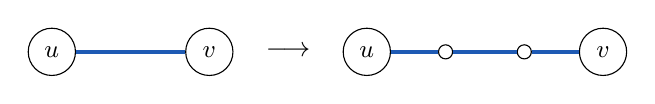
\begin{tikzpicture}\node[lab](u)at(0,0){$u$};\node[lab](v)at(2,0){$v$};\draw[edge](u)--(v);\node at(3,0){$\longrightarrow$};\node[lab](a)at(4,0){$u$};\node[v](b)at(5,0){};\node[v](c)at(6,0){};\node[lab](d)at(7,0){$v$};\draw[edge](a)--(b)--(c)--(d);\end{tikzpicture}\end{center}
Subdivision preserves planarity.
\end{frame}
\begin{frame}{Homeomorphic Graphs}
\large
\Def{Homeomorphic}{Two graphs are homeomorphic if they have isomorphic subdivisions.}
\gap In drawings, a degree-two vertex can be inserted along an edge or suppressed along a path without creating a crossing.
\gap This lets us recognize a nonplanar configuration even when its edges have been stretched into longer paths.
\end{frame}
\begin{frame}{Theorem: Kuratowski's Theorem}
\large
\Thm{Kuratowski}{A finite graph is planar exactly when it contains no subgraph that is a subdivision of $K_5$ or $K_{3,3}$.}
\gap The subdivision need not be induced: extra edges can be ignored.
\gap We use the theorem as a structural criterion; its full sufficiency proof is beyond this lecture.
\end{frame}
\begin{frame}{Why the Forbidden Subdivisions Obstruct Planarity}
\large
\Proof{A subgraph of a planar graph is planar. If a subdivision of $K_5$ or $K_{3,3}$ were planar, suppressing its inserted degree-two vertices would give a plane drawing of $K_5$ or $K_{3,3}$.\gap We have proved that neither graph is planar. Therefore no planar graph can contain either subdivision.\hfill$\square$}
\end{frame}
\begin{frame}{A Subdivision Can Pass the Numerical Tests}
\large
\Example{Subdivide every edge of $K_{3,3}$ once. The resulting graph has $15$ vertices and $18$ edges.}
It satisfies both $18\le3(15)-6$ and $18\le2(15)-4$.
\gap Nevertheless, it is nonplanar: it is itself a subdivision of $K_{3,3}$.
\end{frame}
\begin{frame}{How to Recognize a Subdivision}
\large
\begin{enumerate}\setlength{\itemsep}{.22cm}
\item Identify the branch vertices: five for $K_5$, or two groups of three for $K_{3,3}$.
\item Replace each required edge by a path between its endpoints.
\item Check that these paths have pairwise disjoint interiors.
\item Delete irrelevant edges and vertices.
\end{enumerate}
\gap Paths may meet at required branch vertices, but not at additional internal vertices.
\end{frame}
\begin{frame}{Practice: Prove or Disprove}
\large
\Question{(a) Every graph with at most $3n-6$ edges is planar.\gap (b) Every subgraph of a planar graph is planar.\gap (c) Adding a vertex of degree one preserves planarity.\gap (d) Every planar graph has maximum degree at most five.}
\end{frame}
\begin{frame}{Practice: Answers}
\large
\begin{itemize}\setlength{\itemsep}{.25cm}
\item (a) False: $K_{3,3}$.
\item (b) True: delete the unwanted parts of a plane drawing.
\item (c) True: place the new vertex close to its neighbor.
\item (d) False: the star $K_{1,r}$ is planar for every $r$. The theorem bounds the \emph{minimum} degree, not the maximum.
\end{itemize}
\end{frame}
\begin{frame}{Summary: Planarity}
\large
\begin{itemize}\setlength{\itemsep}{.25cm}
\item A planar graph admits a crossing-free drawing.
\item Euler's formula links vertices, edges, and regions.
\item Face counting gives edge and degree bounds.
\item Euler's formula restricts regular polyhedra to five types.
\item Kuratowski's theorem gives the two subdivision obstructions.
\end{itemize}
\end{frame}
\begin{frame}{Next time: Colorings}\begin{center}{\Huge Colorings}\end{center}\end{frame}
\end{document}